\documentclass{article}
\usepackage{graphicx}
\usepackage{siunitx}
\usepackage{soul}
\usepackage{color}
%cover page
\author{Asad Mohiuddin}
\title{Superconducting and Superinsulating Nanofluids}

%----------------------------------------
\begin{document}

%----------------------------------------
\clearpage \maketitle
\thispagestyle{empty} %pervent page numbering

%----------------------------------------
\newpage \setcounter{page}{1}
\section{Abstract}
	Structure:
	\begin{itemize}
		\item Summary of report
	\end{itemize}

\section{Introduction}
	Structure:
	\begin{itemize}
		\item A bit about Nanofluids
		\item Nanofluid Applications
		\item THW 
		\item reason behind making a THW
	\end{itemize}

Nanometer sized solid particles either metallic or non-metallic that are suspended in a base fluid that form a two-phase mixture are classed as nanofluids. Previous investigations show that a large enhancement of the thermophysical properties of a base fluid (i.e. water or oil) can be achieved by the addition of these nanoparticles. These properties include heat thermal conductivity, thermal diffusivity, convective heat transfer coefficient and viscosity \cite{wong2010applications}. 

Modernised nanotechnology now provides the ability to engineer on a molecular and atomic scale to yield nanosized particles (or nanostructured polymers) that often have atleast one of their principle dimensions bellow 100nm. These additives can be present as types of oxide ceramics (e.g. Al$_{2}$O$_{3}$, CuO) or metal oxides (e.g. alumina, silica), also they can be a chemically stable metals, carbon in various forms or even metal carbides \cite{sheikholeslami2017applications}. In general, it is found that dilute multicomponent fluids of nanofluids, typically with volume fractions of 5-10\%, have been used for the purpose of enhanced thermal performance. This is because the nanosized particles dramatically increase the thermal conductivity of the mixture compared to the pure fluid. The magnitude of this enhancement depend on the volume fraction, shape, size and arrangement of the suspended nanoparticles as well as its thermophysical properties. Dilute concentrations of nanoparticles with as low as 1-5\% vol fractions, have demonstrated a thermal conductivity increase of around 60\% \cite{xuan2000conceptions, kakacc2009review}. In every physical mechanism the properties of a given materiel can change completely as it falls bellow a critical scale. This is where nanofluids exhibit enhanced thermophysical
properties compared to their respective bulk forms \cite{shodhganga2018}.

The mechanics of this enhancement have generally fallen into the classical/continuum bounds given by series and parallel resistances. These bounds are defined by two separate phases of the solid nanoparticles and the liquid medium and the arrangement of the nanoparticles with in the medium. But a small number of experimental result do not fall into these bounds such as helium and hydrogen gas mixtures or the theoretical hard sphere model, which instead exhibit conductivity enhancements above the parallel bounds and dehancement below the series bounds. It is necessary to develop a complete theoretical model that describes the heat transfer phenomenon so it can be manifested for practical applications.

Nanofluids present unique features that have more advantages than from those of the conventional solid + liquid mixtures, in which the solid additive particles have physical dimensions that range from micrometer to millimetres. These mixtures tend to incorporate varity of issues such as eroded pipelines, clogged fluid flow, settling of solid particles and intense pressure drops \cite{xuan2000conceptions}. 

Moore's Law is a well-known phenomenon that states that in highly dense integrated circuits (IC) the total number of transistors will approximately double every two years. Thermal management becomes unrealistic as the density of transistors with in the IC increase, thus a new challenge has appeared in heat transfer: cooling of nano-scale devices. A more efficient and compact design of heat exchangers is required for advanced nanoelectronics, and one way this can be achieved is through nanofluid technology. Development on observing these effects are shown in figure \ref{fig:microprocessor}, the experimental set up contains a microprocessor where the total heat flux, Q, has been specified to a copper heat sink that contains steady laminar forced flow of liquid nanofluids with uniform axial velocity and temperature profiles at the inlet \cite{nguyen_2018}. 
	
	\begin{figure}[h] 
		\centering
		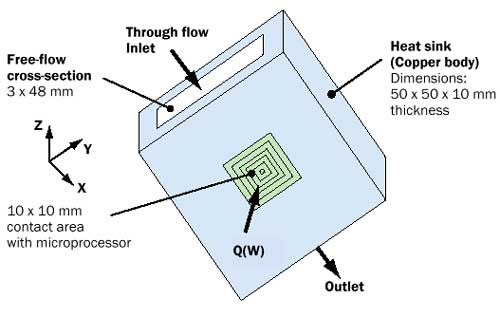
\includegraphics[scale=0.5]{img1}
		\caption{\textit{Nanofluid enhanced heat transfer in microprocessors}}
		\label{fig:microprocessor}
	\end{figure}

Zalman’s company manufactures liquid CPU coolers for high end desktop computers. They are the first company to release a commercial CPU cooler that incorporates nanofluid technology and won a award at CES 2013. The Reserator 3 Max nanofluid cooler shown in figure \ref{fig:CPUcooler}, achieves cooling loads up to 400W while remaining very quiet. The Reserator 3 high-performance pump outputs a flow of 90 litres per hour of nanofluids which contain refrigerant nanoparticles smaller than 100nm, to a dual copper radiator design which feeds into a "quadro cooling path" that consists of two copper pipes sitting behind the fan and encapsulated by radiators \cite{zalman2018}.

	\begin{figure}[h]
		\centering
		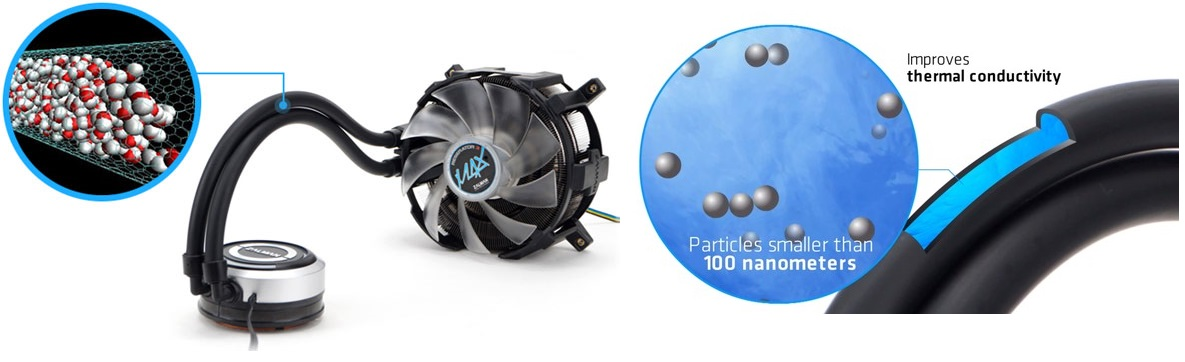
\includegraphics[scale=0.5]{img2}
		\caption{\textit{Nanofluid enhanced heat transfer in CPU coolers}}
		\label{fig:CPUcooler} 
	\end{figure}

Besides the benefits that nanofluids provide for cooling, Iranian researchers from Shiraz University are studying their effect on CO$_{2}$ removal. A CO$_{2}$ separator shown in figure \ref{fig:gasaborber} that contains a gas–liquid hollow fiber membrane contractor uses nanofluids of nanosilica and carbon nanotube as the absorbent. Nanofluid of carbon nanotubes resulted in a enhanced removal efficient of 40\%, compared to that of distilled water \cite{golkhar2013investigation}. Nanofluids could provide good replacement of the usual separating agent or additives to these existing agents to improve CO$_{2}$ absorption. 
	
%	\begin{figure}[h] 
%		\centering
%		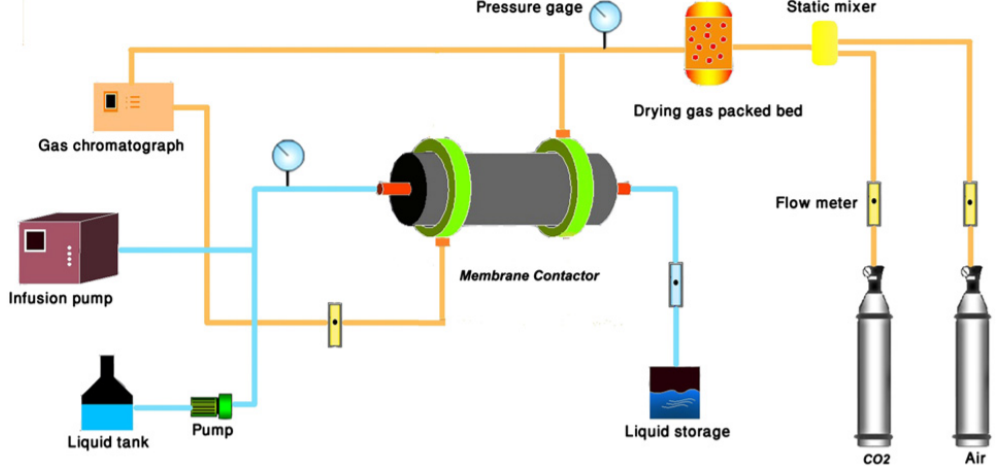
\includegraphics[scale=0.5]{gasabsorber}
%		\caption{\textit{Nanofluids in gas abosrber to improve CO$_{2}$ absorption}}
%		\label{fig:gasaborber}
%	\end{figure}
	
This project explores anomalous heat transfer in nanofluids by their history in thermal conductivity enhancement. This includes describing what models have already been used to approximate their behaviour and critically review their applicability. Perform molecular simulations of thermal conduction to confirm if transient effects in the thermal conductivity, possible at small time/length scales, dominate conduction. This project will also primarily focus on design and construction of a Transient Heated Wire (THW) cell for the testing of liquid and gas mixture thermal conductivities and use this data to explore the anomalous heat transfer in nanofluids and gas mixtures which have similar dimensional properties to nanofluid systems.

Accurate measurements of thermal conductivity of nanofluids are difficult and relatively expensive. Transient hot wire (THW) method is a well established technique to measure thermal conductivity as it is accurate, reliable and robust. \hl{Talk about other techniques to measure thermal conductivity and how they wouldn't work with nanofluids?} A cost effective solution for a design of a precise THW system is by developing it on a Printed Circuit Board (PCB) shown in figure \ref{fig:pcbdesign}, where two platinum wires of a diameter of \SI{1.55}{\micro\metre} is projected through the board. The thermal conductivity is determined by observing the rate at which the temperature profile of the wire increases with time after a step current (or voltage) is applied across it. The wire acts as the heat source and as the temperature sensor, when a known current is applied. The temperature of the wire is found by measuring its resistance using a Wheatstone bridge, where this relationship is well-known.
Taking $ V $ as the voltage across the wire and $ I $ as the current flowing through the wire.

	
	\begin{figure}[h] 
		\centering
		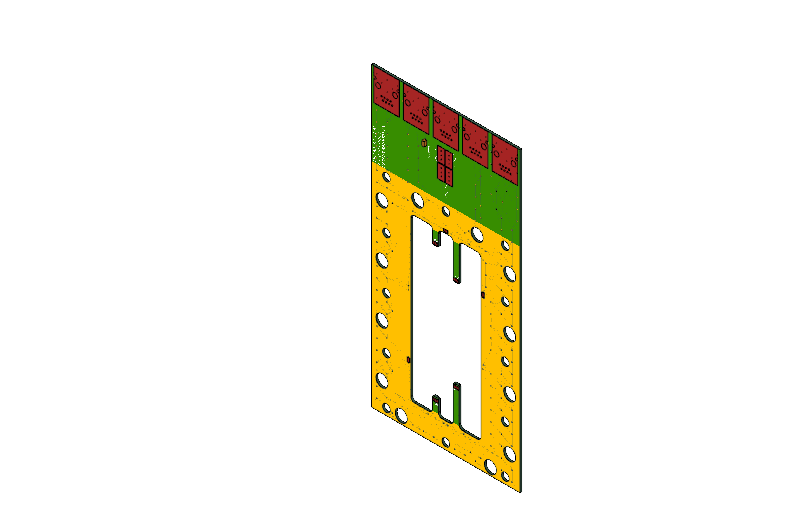
\includegraphics[scale=0.4]{PCBdesign}
		\caption{\textit{THW PCB design}}
		\label{fig:pcbdesign}
	\end{figure}

%----------------------------------------
\newpage
\section{Theory \& Background}
	\subsection{TYPES OF HEAT TRANSFER MECHANISMS}
	Structure:
	\begin{itemize}
		\item Conduction
		\item Convection
		\item Radiation
	\end{itemize}

Heat transfer is an important discipline within thermal engineering, that predicts energy transfer between matter as a result of a driving force from a temperature difference. Just as similar to how an electric potential difference is a driving force for current flow. Heat transfer is a time dependant problem that can provide information on heat exchange rates for specific conditions. There are 3 modes of heat transfer.
 
\subsection{Conduction}
Heat transfer conduction means vibration of atoms that are coupled together. The energy
of the vibrating system is quantised, and phonon is the emission or absorption of quantised
thermal energy by an atom. Therefore, a phonon is essentially a quantised mode of vibration
which plays a main role in the thermal conductivity of a material. A greater phonon density
exists in the hot region than in the cooler one; therefore, heat conduction is essentially due to the diffusion of phonons from the hot region to the cold region \label{}
\subsection{Convection}
\subsection{Radiation}

	
\newpage
	\subsection{HEAT TRANSFER MECHANISMS IN NANOFLUIDS}
	Structure:
	\begin{itemize}
		\item Series parallel 		
		\item Maxwell model	 	
	 	\item Brownian motion of nanoparticles
	 	\item clustering of nanoparticles
	 	\item Interfacial layering of liquid molecules
	 	\item thermophoresis
	\end{itemize}

	\subsection{Series \& Parallel}
	\subsubsection{Series - Upper Limit}
	\subsubsection{Parallel - Lower Limit}
	\subsection{Maxwell's Theory}
	\subsubsection{Upper Bound}
	\subsubsection{Lower Bound}

\newpage	
\section{Transient Heated Wire}
its hard to find solutions to arbitrary integral equations

if its not infentily long then we dont have symmetriay in tat direction, if its not infinitely thin we dont have a boundary condition at one point but its in a shell

%----------------------------------------
\newpage
\section{Transient Heated Wire Design}

%----------------------------------------
\newpage
\bibliography{References}
\bibliographystyle{ieeetr}

%----------------------------------------
\end{document}